
%
%   trk_performance.tex
%       author: Omar Moreno <omoreno1@ucsc.edu>
%      created: December 4, 2012
%
 
A charged particle traversing the sensitive volume of the SVT is expected to
deposit enough charge to produce hits which, in turn, are used to form 
clusters. Clusters which are in adjacent Si planes are then combined to form
2-dimensional ``stereo hits'' which are used by the tracking algorithm to 
form tracks.  The determination of the probability that a stereo hit is 
formed, or hit efficiency, provides insight as to the performance of each of 
the SVT layers.

In order to obtained the hit efficiencies, tracks were fit using only 4 of 
SVT layers. The resulting track was then extrapolated to the layer omitted
\begin{figure}[h]
    \begin{center}
        % TODO: Need to update the plot so that Layer 2 on the bottom doesn't 
        % look terrible. It's probably easiest to just remove the point altogether.
    	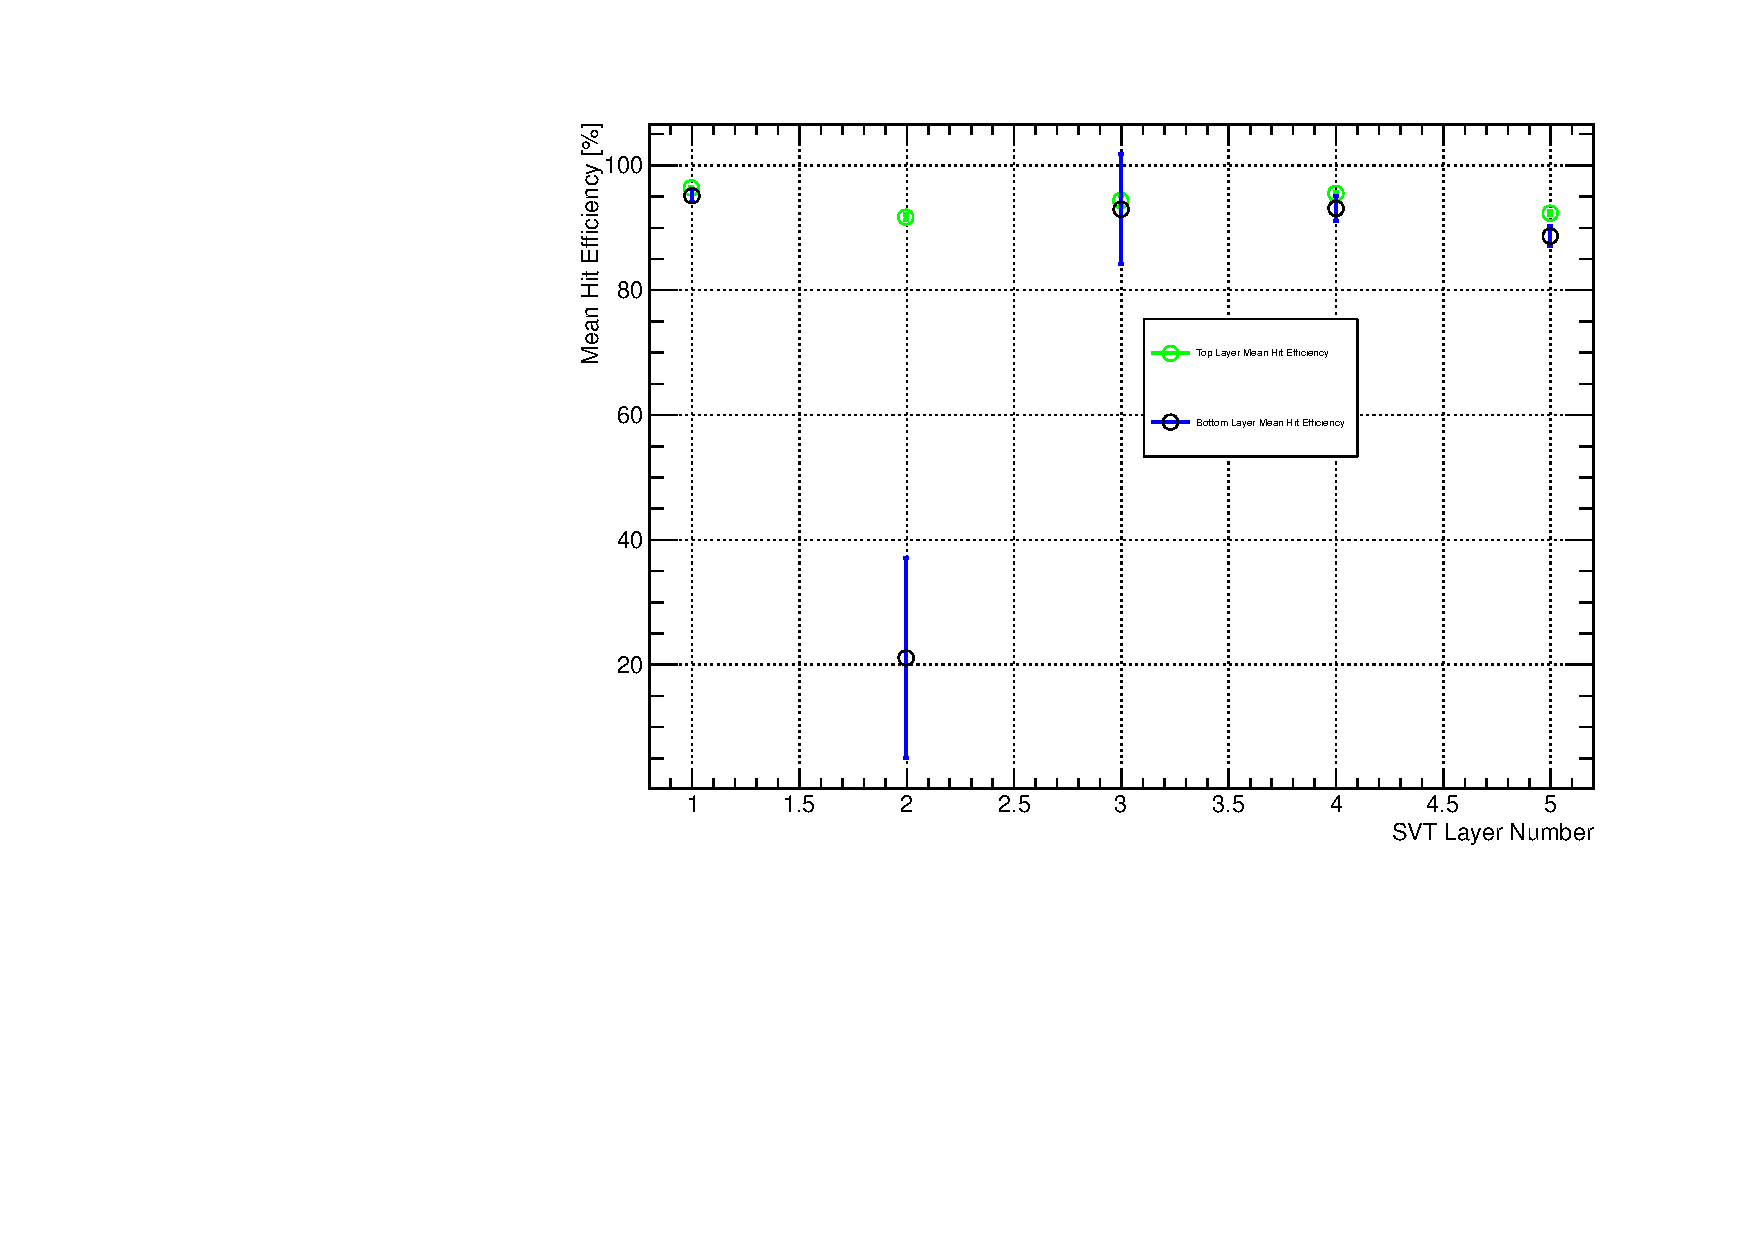
\includegraphics[width=0.49\textwidth]{test2012/svtperformance/trk_performance/mean_hit_efficiency_vs_layer.pdf}
    	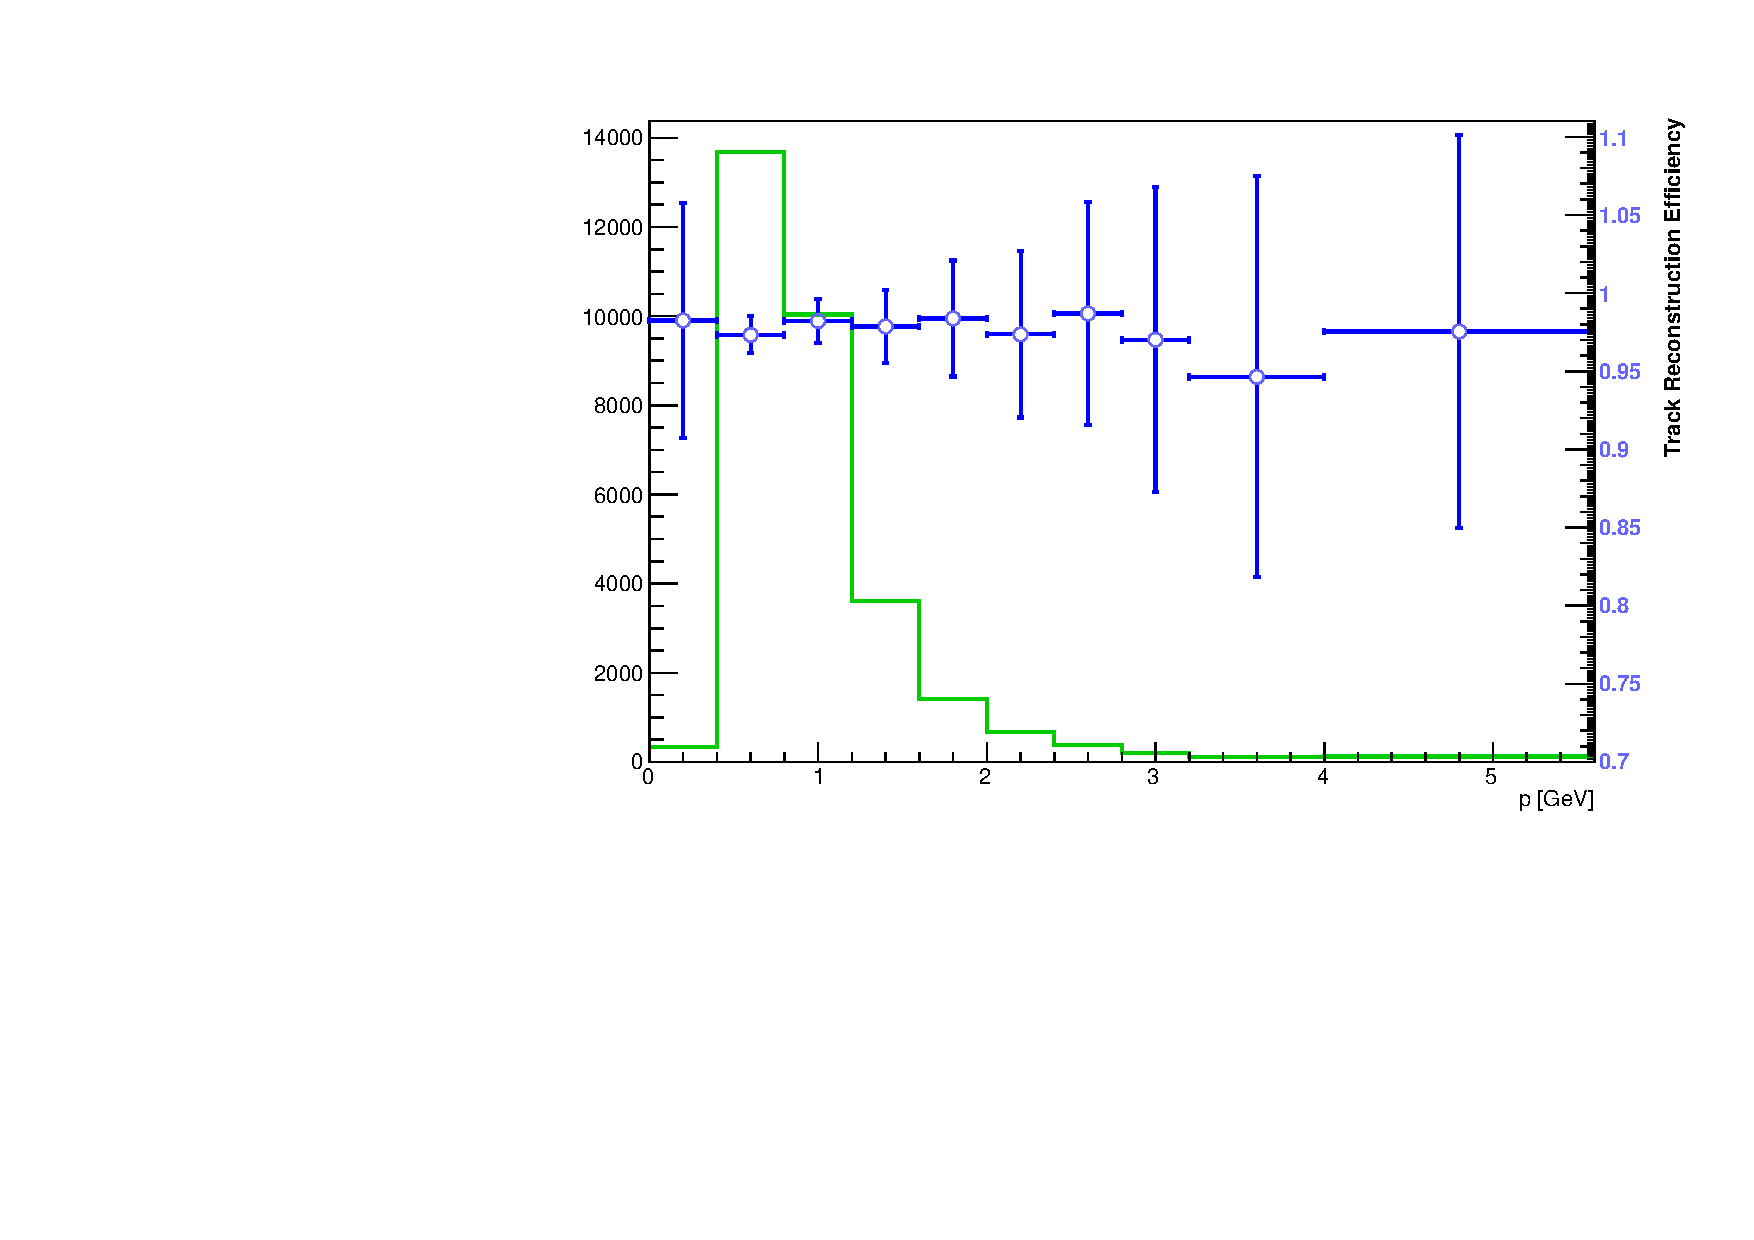
\includegraphics[width=0.49\textwidth]{test2012/svtperformance/trk_performance/track_reco_efficiency.pdf}
        \caption{
                    The plot on the left shows the average hit efficiency
                    from all dedicated photon runs as a function of layer
                    number.  Excluding known bad layers, the hit efficiency
                    is greater than 90\%. The track reconstruction efficiency
                    as a function of momentum (blue) along with the 
                    distribution of momenta for all tracks (green) is shown
                    on the right.
                } 
	\label{fig:hit_track_efficiency}
    \end{center}
\end{figure}
from the fit. If the track was found to lie within the sensitive volume
of the layer, a search for a stereo hit within the layer acceptance was 
conducted.  The hit efficiency was then determined as
\[
    \varepsilon_{\mbox{hit efficiency}} = \frac{\mbox{Tracks with hit on missing layer}}
                                            {\mbox{Tracks within layer acceptance}} \times 100 \%.
\]
The hit efficiencies per layer were calculated using all dedicated runs. As 
can be seen from Figure~\ref{fig:hit_track_efficiency}, the average hit efficiency
per layer, excluding all known bad Si sensors, was found to be greater than
90\%.
% The single hit efficiencies need to be updated to reflect changes that were 
% made to the tracking code

As mentioned above, the standard pattern recognition algorithm is designed to 
find tracks using the reconstructed stereo hits.  A set of tracking strategies
outline which layers should be used by the track finding algorithm along
with their role (seeding, extend, confirm), and the $\chi^2$ cut imposed 
on the fit. Any kinematic constraints are also specified within the strategy.
A detailed account of the tracking algorithm can be found  here~\ref{}.

In order to determine the efficiency of the track finding algorithm, a Monte
Carlo sample containing pair produced electrons from photons incident on 
a 1.6\% $X_0$ gold target was used.  The energy of the pair produced electrons
ranged from .5 GeV to 5.5 GeV. An electron falling within the detector 
acceptance was considered findable by the tracking algorithm if it 
traversed through at least 4 of the SVT layers. The track reconstruction
efficiency was then determined as
\[
    \varepsilon_{\mbox{track reco efficiency}} = \frac{\mbox{Tracks found}}
                                            {\mbox{Tracks found to be findable}} \times 100 \%.
\]
The resulting efficiency to find an electron which passes through the detector
acceptance is show on Figure~\ref{fig:hit_track_efficiency}. The average track
reconstruction efficiency was found to be \% with the bulk of the inefficiency
coming from the $\chi^2$ cut imposed on the fit to the six samples during
the clustering stage.

All events which contained pairs of oppositely charged tracks were fit to a
common vertex using a simple vertexing algorithm which searches for the distance
of closest approach between the two tracks.  The reconstructed vertex position
along the beam axis for both data and Monte Carlo is shown on 
Figure~\ref{fig:vz_position}.
\begin{figure}[h]
    \begin{center}
    	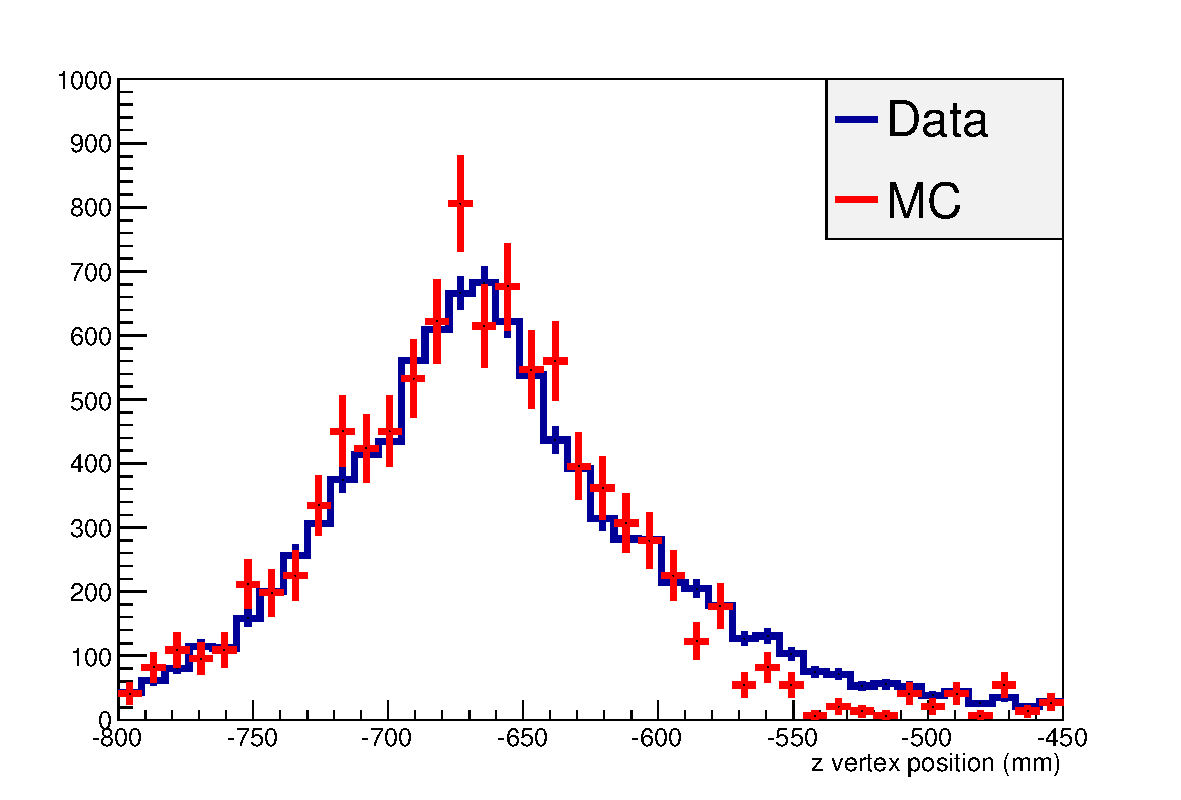
\includegraphics[width=0.60\textwidth]{test2012/svtperformance/trk_performance/zvertex.pdf}
        \caption{  
                    The reconstructed vertex position along the beam axis for
                    both data (blue) and Monte Carlo (red).
                } 
	\label{fig:vz_position}
    \end{center}
\end{figure}
Because of the geometric setup of the SVT, observation of pairs produced by
the incident photon required both electrons to multiple scatter a significant 
amount within the target.  This results in a broadening of the Gaussian 
distributed reconstructed vertex position as seen in the Figure. 

